\documentclass [12pt]{article}
\setlength{\parindent}{0em}
\setlength{\parskip}{0.25in}
\usepackage{geometry}
\geometry{verbose,letterpaper,tmargin=0.5in,bmargin=1.0in,lmargin=.70in,rmargin=.70in}
\usepackage{graphicx}
\usepackage{amsmath}
\usepackage{amssymb}
\usepackage{amsthm}
\theoremstyle{definition}
\newtheorem{exmp}{Example}[section]
\usepackage{tikz}
\usetikzlibrary{arrows,decorations.pathmorphing,backgrounds,positioning,fit,petri,calc,matrix}
\usepackage{slashbox}
\usepackage{listings}
\usepackage{ dsfont }
\usepackage{ upgreek }
\usepackage{graphicx}
\graphicspath{ {./images/} }


\newcommand{\ket}[1]{| {#1} \rangle}
\newcommand{\bra}[1]{\langle {#1} |}
\newcommand{\braket}[2]{\langle #1 \ | \ #2 \rangle}
\newcommand{\qp}[2]{\langle #1 \ | \ #2 \ | \ #1 \rangle}
\newcommand{\tensor}[2]{ #1 \otimes  #2 }
\newcommand{\iz}[1]{\mathds{#1}^{n}}
\newcommand{\md}[1]{|#1|}
\newcommand{\suml}[2]{\sum\limits_{#1}^{#2}}

\definecolor{dkgreen}{rgb}{0,0.6,0}
\definecolor{gray}{rgb}{0.5,0.5,0.5}
\definecolor{mauve}{rgb}{0.58,0,0.82}

\lstset{frame=tb,
  language=Python,
  aboveskip=3mm,
  belowskip=3mm,
  showstringspaces=false,
  columns=flexible,
  basicstyle={\small\ttfamily},
  numbers=none,
  numberstyle=\tiny\color{gray},
  keywordstyle=\color{blue},
  commentstyle=\color{dkgreen},
  stringstyle=\color{mauve},
  breaklines=true,
  breakatwhitespace=true,
  tabsize=3
}

\DeclareMathOperator{\Cspan}{ \CC-span }

\title{Home Work 12}
\author{Madhu Peduri}
\date{05/04/2021}

\begin{document}
\section*{Homework 12}

{\bf 1.} Prove that $\mathcal{P}\ket{x,u} = \ket{x} \otimes U^{[x]}\ket{u}$

\phantom{1em} {\bf 1.} Consider the single, k, unit of the circuit\\
\phantom{1000em} 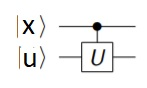
\includegraphics[width=2cm, height=2cm]{I1}

\phantom{1em} {\bf 2.} This is a controlled gate operation on vector $\ket{x}$ with operator $U$

\phantom{1000em} $\wedge(u)\ket{i,\alpha} = 
	\begin{cases}
   		\ket{i} \otimes u\ket{\alpha} & \text{if } i = 1, \\
     	\ket{i,\alpha} = \ket{i} \otimes \ket{\alpha} & \text{otherwise}.
    \end{cases}$

\phantom{1em} {\bf 3.} We can write the output of $k^{th}$ unit as,

\phantom{1000em} $\mathcal{P}\ket{x_{k},u} = 
	\begin{cases}
   		\ket{1} \otimes u^{2^{k}}\ket{u} & \text{if } x = 1, \\
     	\ket{0} \otimes \ket{u} & \text{if } x = 0.
    \end{cases}$

\phantom{1000em} $\mathcal{P}\ket{x_{k},u} = \ket{x_{k}} \otimes U^{2^{k}x_{k}}\ket{u}$

\phantom{1em} {\bf 4.} We can write the output for the full circuit as below,

\phantom{1000em} $\mathcal{P}\ket{x,u} = (\ket{x_{0}} \otimes U^{2^{n-1}x_{0}}\ket{u}) \otimes (\ket{x_{1}} \otimes U^{2^{n-2}x_{1}}\ket{u}) \otimes \dots \otimes (\ket{x_{n-1}} \otimes U^{2^{0}x_{n-1}}\ket{u})$

\phantom{1000em} $ = \ket{x_{0}} \otimes \ket{x_{1}} \otimes \dots \otimes \ket{x_{n-1}} \otimes U^{2^{n-1}x_{0}} . U^{2^{n-2}x_{1}} . \dots . U^{2^{0}x_{n-1}} . \ket{u}$

\phantom{1000em} $ = \ket{x_{0}} \otimes \ket{x_{1}} \otimes \dots \otimes \ket{x_{n-1}} \otimes e^{i2\Uppi2^{n-1}x_{0}} . e^{i2\Uppi2^{n-2}x_{1}} . \dots . e^{i2\Uppi2^{0}x_{n-1}} . \ket{u}$

\phantom{1000em} $ = \ket{x_{0}} \otimes \ket{x_{1}} \otimes \dots \otimes \ket{x_{n-1}} \otimes e^{i2\Uppi[2^{n-1}x_{0}+2^{n-2}x_{1}+2^{0}x_{n-1}]} . \ket{u}$

\phantom{1000em} $ =\ket{x} \otimes U^{[x]} \otimes \ket{u}$, where $[x]$ is the number with binary representation x

\newpage

{\bf 2.} Prove that $\braket{\alpha}{\beta} = 0$ and $\ket{\alpha}, \ket{\beta}$ are orthogonal

\phantom{1em} {\bf 1.} We have $U$ as the unitary operator for the eigenvectors $\ket{\alpha}, \ket{\beta}$ with eigenvalues $\lambda, \upmu$

\phantom{1000em} $\Rightarrow U\ket{\alpha} = \lambda\ket{\alpha} \Rightarrow \bra{\alpha}U^{\dagger} = \bra{\alpha}\lambda$

\phantom{1000em} Similarly, $\Rightarrow U\ket{\beta} = \upmu\ket{\beta} \Rightarrow \bra{\beta}U^{\dagger} = \bra{\beta}\upmu$

\phantom{1em} {\bf 2.} From above equations, we can say that

\phantom{1000em} $\bra{\alpha} U U^{\dagger} \ket{\beta} = \bra{\alpha} \lambda \upmu \ket{\beta}$
 
\phantom{1000em} As $U$ is a unitary operator, $U.U^{\dagger} = 1$\\
\phantom{1000em} $\Rightarrow \braket{\alpha}{\beta} = \lambda\upmu \braket{\alpha}{\beta}$

\phantom{1em} {\bf 3.} If $\braket{\alpha}{\beta} \neq 0$, then \\
\phantom{1000em} $\lambda = \upmu = 1$  or $\upmu = \bar{\lambda}$, where $\lambda, \upmu \in \mathds{C}$ of the form $e^{i2\Uppi \frac{k}{t}}$\\
\phantom{1000em} But this is against the given condition $\lambda \neq \upmu$

\phantom{1em} {\bf 4.} So, if $\lambda \neq \upmu$, then,\\
\phantom{1000em} $\braket{\alpha}{\beta} = \lambda\upmu \braket{\alpha}{\beta} = 0$ \\
\phantom{1000em}$\Rightarrow \ket{\alpha}, \ket{\beta}$ are orthogonal

{\bf 3.} Show that $\hat{l_{\oplus}}(\ket{\psi} \otimes \ket{0}) = \ket{\psi} \otimes \ket{\psi} \Leftrightarrow \ket{\psi} = \ket{0}$ or $\ket{\psi} = \ket{1}$ 

\phantom{1em} {\bf 1.} Suppose, $\hat{l_{\oplus}}$ is the quantumn clone operator,

\phantom{1000em} $\Rightarrow \hat{l_{\oplus}}\ket{0}\ket{0} = \ket{0}\ket{0}$ and $\hat{l_{\oplus}}\ket{1}\ket{0} = \ket{1}\ket{1}$ 

\phantom{1em} {\bf 2.} Let us consider the qubit in the state $\ket{\psi} = \dfrac{1}{\sqrt{2}}(\ket{0} + \ket{1})$ 

\phantom{1000em} if we apply the clone operator on $\psi$, by linearity, \\
\phantom{1000em} $\hat{l_{\oplus}}\ket{\psi}\ket{0} = \hat{l_{\oplus}}\dfrac{1}{\sqrt{2}}(\ket{0} + \ket{1})\ket{0}$ \\
\phantom{1000em} $ = \dfrac{1}{\sqrt{2}}(\hat{l_{\oplus}}\ket{0}\ket{0} + \hat{l_{\oplus}}\ket{1}\ket{0})$\\
\phantom{1000em} $ = \dfrac{1}{\sqrt{2}}(\ket{0}\ket{0} +\ket{1}\ket{1})$\\
\phantom{1000em} $ \neq \dfrac{1}{\sqrt{2}}(\ket{0} + \ket{1})\dfrac{1}{\sqrt{2}}(\ket{0} + \ket{1}) \neq \dfrac{1}{2}(\ket{00} + \ket{10} + \ket{01} + \ket{11})$

\phantom{1em} {\bf 3.} Thus, cloning operator $\hat{l_{\oplus}}$ work if $\ket{01} = \ket{10} = 0$. \\
\phantom{1000em} $\Rightarrow$ only if $\ket{\psi} = \ket{0}$ or $\ket{1}$

\newpage

{\bf 4.} Show that $U$ clones $\ket{\varphi}$ and $\ket{\psi}$ if and only if $\ket{\varphi} = \ket{\psi}$ or $\braket{\varphi}{\psi} = 0$ 

\phantom{1em} {\bf 1.} Given cloning is a unitary transformation, which should preserve the geometry of the vectors. \\
\phantom{1000em} We use inner product to verify. Inner product should be same (preserves geometry) \\
\phantom{1000em} for given equations,

\phantom{1000em} $U(\ket{\varphi} \otimes \ket{0^{n}}) = \ket{\varphi} \otimes \ket{\varphi}$, $U(\ket{\psi} \otimes \ket{0^{n}}) = \ket{\psi} \otimes \ket{\psi}$

\phantom{1em} {\bf 2.} $(\bra{\varphi} \otimes \bra{0^{n}})U^{\dagger}U(\ket{\varphi} \otimes \ket{0^{n}})$

\phantom{1000em} $= (\bra{\varphi} \otimes \bra{0^{n}})(\ket{\varphi} \otimes \ket{0^{n}}) = \braket{\varphi}{\psi}\braket{0^{n}}{0^{n}} - 1$

\phantom{1em} {\bf 3.} $(\bra{\varphi} \otimes \bra{\varphi})(\ket{\psi} \otimes \ket{\psi})$

\phantom{1000em} $= \braket{\varphi}{\psi}\braket{\varphi}{\psi} - 2$

\phantom{1em} {\bf 4.} Equation 1 and 2 are equal,

\phantom{1000em} $\braket{\varphi}{\psi}\braket{0^{n}}{0^{n}} = \braket{\varphi}{\psi}\braket{\varphi}{\psi}$

\phantom{1000em} if and only if\\
\phantom{1000em} $\Rightarrow \braket{\varphi}{\psi} = 0 $\\
\phantom{1000em} $\Rightarrow \ket{\varphi} \ket{\psi}$ are orthogonal  

\phantom{1000em} or\\
\phantom{1000em} $\Rightarrow \braket{\varphi}{\psi} = 1$\\
\phantom{1000em} $\Rightarrow \ket{\varphi} = \ket{\psi}$

{\bf 5.} Show that, Quantum cloning operators do not work for all pair of states

\phantom{1em} {\bf 1.} Let us consider the qubit in the state $\ket{\psi} = \dfrac{1}{\sqrt{2}}(\ket{0} + \ket{1})$ \\
\phantom{1000em} if we apply the clone operator on $\psi$, by linearity, \\
\phantom{1000em} $\hat{l_{\oplus}}(\ket{\psi} \otimes \ket{0}) = \hat{l_{\oplus}}\dfrac{1}{\sqrt{2}}(\ket{0} + \ket{1})\ket{0}$ \\
\phantom{1000em} $ = \dfrac{1}{\sqrt{2}}(\hat{l_{\oplus}}\ket{0}\ket{0} + \hat{l_{\oplus}}\ket{1}\ket{0})$\\
\phantom{1000em} $ = \dfrac{1}{\sqrt{2}}(\ket{0}\ket{0} +\ket{1}\ket{1})$

\phantom{1000em} $ \ket{\psi} \otimes \ket{\psi} = \dfrac{1}{\sqrt{2}}(\ket{0} + \ket{1})\dfrac{1}{\sqrt{2}}(\ket{0} + \ket{1}) = \dfrac{1}{2}(\ket{00} + \ket{10} + \ket{01} + \ket{11})$

\phantom{1em} {\bf 2.} $\Rightarrow \hat{l_{\oplus}}(\ket{\psi} \otimes \ket{0}) \neq \ket{\psi} \otimes \ket{\psi}$ Cloning failed on this pair of state.

\end{document}